%%% Hlavní soubor. Zde se definují základní parametry a odkazuje se na ostatní části. %%%

%% Verze pro jednostranný tisk:
% Okraje: levý 40mm, pravý 25mm, horní a dolní 25mm
% (ale pozor, LaTeX si sám přidává 1in)
\documentclass[12pt,a4paper]{report}
\setlength\textwidth{145mm}
\setlength\textheight{247mm}
\setlength\oddsidemargin{15mm}
\setlength\evensidemargin{15mm}
\setlength\topmargin{0mm}
\setlength\headsep{0mm}
\setlength\headheight{0mm}
% \openright zařídí, aby následující text začínal na pravé straně knihy
\let\openright=\clearpage


%%% Údaje o práci

% Název práce v jazyce práce (přesně podle zadání)
\def\NazevPrace{Analyzing Data Lineage in Database Frameworks}
% Jméno autora
\def\AutorPrace{Richard Eliáš}
% Rok odevzdání
\def\RokOdevzdani{2019}
% Název katedry nebo ústavu, kde byla práce oficiálně zadána
% (dle Organizační struktury MFF UK, případně plný název pracoviště mimo MFF)
\def\Katedra{Department of Distributed and Dependable Systems}
% Jedná se o katedru (department) nebo o ústav (institute)?
\def\TypPracoviste{Department}
% Vedoucí práce: Jméno a příjmení s~tituly
\def\Vedouci{RNDr. Pavel Parízek, Ph.D.}
% Pracoviště vedoucího (opět dle Organizační struktury MFF)
\def\KatedraVedouciho{Department of Distributed and Dependable Systems}
% Studijní program a obor
\def\StudijniProgram{Computer Science}
\def\StudijniObor{Artificial Inteligence}
% Nepovinné poděkování (vedoucímu práce, konzultantovi, tomu, kdo
% zapůjčil software, literaturu apod.)
\def\Podekovani{%
  TODO Podakovanie
}
% Abstrakt (doporučený rozsah cca 80-200 slov; nejedná se o zadání práce)
\def\Abstrakt{%
  TODO Abstrakt
}
% 3 až 5 klíčových slov (doporučeno), každé uzavřeno ve složených závorkách
\def\KlicovaSlova{%
  TODO Klucove slova
}


\usepackage{filecontents}
\begin{filecontents*}{\jobname.xmpdata}
  \Author{\AutorPrace}
  \Title{\NazevPrace}
  \Keywords{\KlicovaSlova}
  \Subject{\Abstrakt}
  \Publisher{Univerzita Karlova}
\end{filecontents*}

%% Vytváříme PDF/A-2u
\usepackage[a-2u]{pdfx}

\usepackage{lmodern}
\usepackage[T1]{fontenc}
\usepackage{textcomp}

%% Použité kódování znaků: obvykle latin2, cp1250 nebo utf8:
\usepackage[utf8]{inputenc}

%%% Další užitečné balíčky (jsou součástí běžných distribucí LaTeXu)
\usepackage{amsmath}        % rozšíření pro sazbu matematiky
\usepackage{amsfonts}       % matematické fonty
\usepackage{amsthm}         % sazba vět, definic apod.
\usepackage{bbding}         % balíček s nejrůznějšími symboly
			    % (čtverečky, hvězdičky, tužtičky, nůžtičky, ...)
\usepackage{bm}             % tučné symboly (příkaz \bm)
\usepackage{graphicx}       % vkládání obrázků
\usepackage{fancyvrb}       % vylepšené prostředí pro strojové písmo
\usepackage{indentfirst}    % zavede odsazení 1. odstavce kapitoly
\usepackage[numbers]{natbib}         % zajištuje možnost odkazovat na literaturu
			    % stylem AUTOR (ROK), resp. AUTOR [ČÍSLO]
\usepackage[nottoc]{tocbibind} % zajistí přidání seznamu literatury,
                            % obrázků a tabulek do obsahu
\usepackage{icomma}         % inteligetní čárka v matematickém módu
\usepackage{dcolumn}        % lepší zarovnání sloupců v tabulkách
\usepackage{booktabs}       % lepší vodorovné linky v tabulkách
\usepackage{paralist}       % lepší enumerate a itemize
\usepackage{float}

\usepackage{subcaption}
\usepackage[noend]{algpseudocode}
\usepackage{algorithm}
\usepackage{cases}
\usepackage{tikz}
\usepackage{amssymb}
\usepackage{xspace}

\usepackage[percent]{overpic}

\usepackage{listings}
\usepackage{color}


%% Balíček hyperref, kterým jdou vyrábět klikací odkazy v PDF,
%% ale hlavně ho používáme k uložení metadat do PDF (včetně obsahu).
\hypersetup{unicode}
\hypersetup{breaklinks=true}
\hypersetup{urlcolor=blue}

%% Definice různých užitečných maker (viz popis uvnitř souboru)
%%% Tento soubor obsahuje definice různých užitečných maker a prostředí %%%
%%% Další makra připisujte sem, ať nepřekáží v ostatních souborech.     %%%

%%% Drobné úpravy stylu

% Tato makra přesvědčují mírně ošklivým trikem LaTeX, aby hlavičky kapitol
% sázel příčetněji a nevynechával nad nimi spoustu místa. Směle ignorujte.
\makeatletter
\def\@makechapterhead#1{
  {\parindent \z@ \raggedright \normalfont
   \Huge\bfseries \thechapter. #1
   \par\nobreak
   \vskip 20\p@
}}
\def\@makeschapterhead#1{
  {\parindent \z@ \raggedright \normalfont
   \Huge\bfseries #1
   \par\nobreak
   \vskip 20\p@
}}
\makeatother

% Toto makro definuje kapitolu, která není očíslovaná, ale je uvedena v obsahu.
\def\chapwithtoc#1{
\chapter*{#1}
\addcontentsline{toc}{chapter}{#1}
}

% Trochu volnější nastavení dělení slov, než je default.
\lefthyphenmin=2
\righthyphenmin=2

% Zapne černé "slimáky" na koncích řádků, které přetekly, abychom si
% jich lépe všimli.
\overfullrule=1mm

%%% Makra pro definice, věty, tvrzení, příklady, ... (vyžaduje baliček amsthm)

\theoremstyle{plain}
\newtheorem{veta}{Veta}
\newtheorem{lemma}[veta]{Lemma}
\newtheorem{tvrz}[veta]{Tvdenie}

\theoremstyle{plain}
\newtheorem{definice}{Definícia}

\theoremstyle{remark}
\newtheorem*{dusl}{Dôsledok}
\newtheorem*{pozn}{Poznámka}
\newtheorem*{prikl}{Príklad}

%%% Prostředí pro důkazy

\newenvironment{dukaz}{
  \par\medskip\noindent
  \textit{Dôkaz}.
}{
\newline
\rightline{$\square$}  % nebo \SquareCastShadowBottomRight z balíčku bbding
}

%%% Prostředí pro sazbu kódu, případně vstupu/výstupu počítačových
%%% programů. (Vyžaduje balíček fancyvrb -- fancy verbatim.)

\DefineVerbatimEnvironment{code}{Verbatim}{fontsize=\small, frame=single}

%%% Prostor reálných, resp. přirozených čísel
\newcommand{\R}{\mathbb{R}}
\newcommand{\N}{\mathbb{N}}

%%% Užitečné operátory pro statistiku a pravděpodobnost
\DeclareMathOperator{\pr}{\textsf{P}}
\DeclareMathOperator{\E}{\textsf{E}\,}
\DeclareMathOperator{\var}{\textrm{var}}
\DeclareMathOperator{\sd}{\textrm{sd}}

%%% Příkaz pro transpozici vektoru/matice
\newcommand{\T}[1]{#1^\top}

%%% Vychytávky pro matematiku
\newcommand{\goto}{\rightarrow}
\newcommand{\gotop}{\stackrel{P}{\longrightarrow}}
\newcommand{\maon}[1]{o(n^{#1})}
\newcommand{\abs}[1]{\left|{#1}\right|}
\newcommand{\dint}{\int_0^\tau\!\!\int_0^\tau}
\newcommand{\isqr}[1]{\frac{1}{\sqrt{#1}}}

%%% Vychytávky pro tabulky
\newcommand{\pulrad}[1]{\raisebox{1.5ex}[0pt]{#1}}
\newcommand{\mc}[1]{\multicolumn{1}{c}{#1}}

\renewcommand{\O}[1]{\sloppy\mbox{\ensuremath{\mathcal{O}}(#1)}}

\newcommand{\scale}{0.6}
\newcommand{\subtree}[1]{\begin{tikzpicture}[
          on grid,
          font=\tiny,
          scale = \scale,
          node distance = 0.6 cm,
          sibling distance = 0.8 cm,
          text width = 0.2cm,
          level distance = 1.1 cm,
          colored/.style = {color = red},
          normal/.style = {black = red, draw, opacity = 100},
          invisible/.style={opacity = 0},
          cross/.style={path picture={ 
                \draw
                (path picture bounding box.south east) -- (path picture bounding box.north west) (path picture bounding box.south west) -- (path picture bounding box.north east);
            }},
          every node/.style = {scale = \scale, circle, draw, align = center},
          tree/.style = {draw = none, fill = none}]#1\end{tikzpicture}}

\definecolor{green}{rgb}{0,0.6,0}
\definecolor{gray}{rgb}{0.5,0.5,0.5}
\definecolor{yellow}{rgb}{0.73,0.71,0.16}
\definecolor{pink}{rgb}{0.58,0,0.82}
\definecolor{orange}{rgb}{0.8,0.47,0.19}

\lstdefinelanguage{Java}{
  morekeywords={
    return,try,catch,finally,
    static,default,final,volatile,new,
    null,void,int,long,boolean,short,double,float,
    interface,class,extends,implements,
    if,else,for,while,do,throw,throws,
    public,protected,private},
  numbers=left,
  numbersep=3mm,
  numberstyle=\tiny\color{gray},
  frame=tb,
  %aboveskip=3mm,
  %belowskip=3mm,
  showstringspaces=false,
  columns=flexible,
  basicstyle={\footnotesize\ttfamily},
  showlines=false,
  keywordstyle=\color{blue},
  commentstyle=\color{green},
  morecomment=[l]{//},
  morecomment=[s]{/*}{*/},
  stringstyle=\color{pink},
  morestring=[b]",
  morestring=[d]’,
  moredelim=[is][\textcolor{yellow}]{@@}{@@},
  breaklines=true,
  breakatwhitespace=true,
  escapeinside={/*}{*/},
  captionpos=b,
}

\lstdefinelanguage{XML}{
  %language=HTML,
  numbers=left,
  numbersep=3mm,
  numberstyle=\tiny\color{gray},
  frame=tb,
  %aboveskip=3mm,
  %belowskip=3mm,
  showstringspaces=false,
  columns=flexible,
  basicstyle={\footnotesize\ttfamily},
  showlines=false,
  keywordstyle=\color{blue},
  commentstyle=\color{green},
  morecomment=[s]{<!--}{-->},
  stringstyle=\color{pink},
  moredelim=[is][\textcolor{blue}]{@}{@},
  moredelim=[is][\textcolor{orange}]{@@}{@@},
  morestring=[b]",
  morestring=[d]’,
  breaklines=true,
  breakatwhitespace=true,
  escapeinside={/*}{*/},
  captionpos=b,
}

\makeatletter
\AtBeginDocument{%
  \let\c@table\c@lstlisting
  \let\thetable\thelstlisting

  \let\c@figure\c@lstlisting
  \let\thefigure\thelstlisting
  \let\ftype@lstlisting\ftype@figure
}
\makeatother

\newcommand\TODO[1]{{\color{red}TODO #1}}
\newcommand{\uvodzovky}[1]{``#1''}



%% Titulní strana a různé povinné informační strany
\begin{document}
%%% Title page of the thesis and other mandatory pages

%%% Title page of the thesis

\pagestyle{empty}
\hypersetup{pageanchor=false}
\begin{center}

\centerline{\mbox{
\includegraphics[width=166mm]{img/logo-en.pdf}}}

\vspace{-8mm}
\vfill

{\bf\Large MASTER THESIS}

\vfill

{\LARGE\AutorPrace}

\vspace{15mm}

{\LARGE\bfseries\NazevPrace}

\vfill

\Katedra

\vfill

\begin{tabular}{rl}
Supervisor of the master thesis: & \Vedouci \\
\noalign{\vspace{2mm}}
Study programme: & \StudijniProgram \\
\noalign{\vspace{2mm}}
Study branch: & \StudijniObor \\
\end{tabular}

\vfill

% Zde doplňte rok
Prague \RokOdevzdani

\end{center}

\newpage

%%% Here should be a bound sheet included -- a signed copy of the "master
%%% thesis assignment". This assignment is NOT a part of the electronic
%%% version of the thesis. DO NOT SCAN.

%%% A page with a solemn declaration to the master thesis

\openright
\hypersetup{pageanchor=true}
\pagestyle{plain}
\pagenumbering{roman}
\vglue 0pt plus 1fill

I~hereby declare that I~have authored this thesis independently,
and that all sources used are declared in accordance with the
\uvodzovky{Metodický pokyn o~etické přípravě vysokoškolských závěrečných prací}.

\vspace{2mm}
I~acknowledge that my thesis (work) is subject to the rights and obligations
arising from Act No. 121/2000 Coll., on Copyright and Rights Related to Copyright
and on Amendments to Certain Laws (the Copyright Act), as amended,
(hereinafter as the "Copyright Act"), in particular §~35, and §~60 of the Copyright Act
governing the school work.

\vspace{2mm}
With respect to the computer programs that are part of my thesis (work)
and with respect to all documentation related to the computer programs ("software"),
I~hereby grant the so-called MIT License.

\vspace{2mm}
The MIT License represents a~license to use the software free of charge.
I~grant this license to every person interested in using the software.
Each person is entitled to obtain a~copy of the software (including
the related documentation) without any limitation, and may, without limitation,
use, copy, modify, merge, publish, distribute, sublicense and~/~or sell
copies of the software, and allow any person to whom the software is further
provided to exercise the aforementioned rights. Ways of using the software or the extent
of this use are not limited in any way.

\vspace{2mm}
The person interested in using the software is obliged to attach the text of the license terms as follows:

\vspace{3mm}
\noindent
Copyright (c) \RokOdevzdani~\AutorPrace \\
Permission is hereby granted, free of charge, to any person \\
obtaining a copy of this software and associated documentation \\
files (the \uvodzovky{Software}), to deal in the Software without \\
restriction, including without limitation the rights to use, \\
copy, modify, merge, publish, distribute, sublicense, and/or sell \\
copies of the Software, and to permit persons to whom the \\
Software is furnished to do so, subject to the following conditions: \\
The above copyright notice and this permission notice shall be \\
included in all copies or substantial portions of the Software.

{
\footnotesize
\vspace{3mm}
\noindent
THE SOFTWARE IS PROVIDED \uvodzovky{AS IS}, WITHOUT WARRANTY OF ANY KIND, \\
EXPRESS OR IMPLIED, INCLUDING BUT NOT LIMITED TO THE WARRANTIES \\
OF MERCHANTABILITY, FITNESS FOR A PARTICULAR PURPOSE AND \\
NONINFRINGEMENT. IN NO EVENT SHALL THE AUTHORS OR COPYRIGHT \\
HOLDERS BE LIABLE FOR ANY CLAIM, DAMAGES OR OTHER LIABILITY, \\
WHETHER IN AN ACTION OF CONTRACT, TORT OR OTHERWISE, ARISING \\
FROM, OUT OF OR IN CONNECTION WITH THE SOFTWARE OR THE USE OR \\
OTHER DEALINGS IN THE SOFTWARE.
}

\vspace{15mm}

\hbox{\hbox to 0.5\hsize{%
In $\ldots\ldots\ldots$ date $\ldots\ldots\ldots$
\hss}}

\vspace{20mm}
\newpage

%%% Podekovani

\openright

\Podakovanie

\newpage

%%% Mandatory information page of the thesis

\openright

\vbox to 0.5\vsize{
\setlength\parindent{0mm}
\setlength\parskip{5mm}

Title:
\NazevPrace

Author:
\AutorPrace

\TypPracoviste:
\Katedra

Supervisor:
\Vedouci, \KatedraVedouciho

Abstract:
\Abstrakt

Keywords:
\KlicovaSlova

\vss}

\newpage

\openright
\pagestyle{plain}
\pagenumbering{arabic}
\setcounter{page}{1}



%%% Strana s automaticky generovaným obsahem bakalářské práce

\tableofcontents

%%% Jednotlivé kapitoly práce jsou pro přehlednost uloženy v samostatných souborech

\chapter{Introduction}

For modern data processing applications, an important aspect
is a data lineage.
Data lineage, or provenance, describes where data came from,
how it was derived and where the results are stored.

Lineage can be useful in many domains.
Molecular biology databases, which mostly store copied data,
can use lineage to verify the copied data by tracking the original
sources as was demonstrated by \citet{DataLineageInBioInformatics}.
Probabilistic databases can exploit lineage for confidence
computation as was stated by \citet{DataLineageInProbabilisticDatabases}.
The important usage of the data lineage is also in machine learning,
where for the purpose of a verification and validation can be important
to know data sources of used data sets.
Data lineage is also important in Business Intelligence (BI)
when achieving full regulatory compliance and improving data governance.

In all these areas, Java applications together with data manipulation frameworks
are often used to access data in databases, files or in network storages.
The tool that is able to identify the sources and sinks of a data
and create data lineage of an application can be very useful.

Up to now, we are aware of the only tool for creating data lineage of
Java applications - the Symbolic analysis library
presented in \citet{ParizekHybridAnalysis}.
The library can create data lineage of an analysed application when only
Java I/O and JDBC APIs are used in addition to the core
Java libraries (collections, etc.).



\section{MANTA Flow}

An example of a data lineage analysis tool is the \citet{MantaFlow}.
The MANTA Flow helps enterprises to get end-to-end
data lineage including custom SQL code. That allows customers to fulfill
compliance regulations or improve data governance.

It extracts and analyses metadata from report definitions,
custom SQL code, and extract-transform-load (ETL) workflows, to create data flow graphs
which span multiple systems and a range of technologies.
Lineages are computed based on analysis of actual code.
All entities detected by MANTA Flow, such as database tables, columns or procedures,
are visualized to help users utilize this information.

Systems, for which MANTA Flow is used to analyse their data lineage,
often use Java applications and data processing frameworks to work with data.
MANTA Flow integrates the Symbolic analysis library to create data lineage of
Java applications to cover whole system, not only its database parts.
However, the support for computing data lineage of complex data processing frameworks
is missing.




\section{Goals}

In our work, we \textit{propose architecture changes} to Symbolic analysis library
to be easily extensible by plugins that can add support for new data processing frameworks
to identify its data sources and sinks.

We also \textit{implement Symbolic analysis library plugins} for few selected frameworks
(MyBatis, Spring JDBC and Apache Kafka).
Each framework has different approach for accessing the data.
Thereby we want to demonstrate that such plugins can be used to
add support for data lineage analysis of other Java frameworks.
The feature to easily extend the Symbolic analysis library to add support for a new frameworks
is very important, as new frameworks are being developed today.




\section{Structure of the Work}

The rest of the thesis has the following structure.

In chapter \ref{chapter:frameworks} we give overview of popular Java frameworks
for data processing.

In chapter \ref{chapter:analysis} we introduce libraries that are used
for static analysis of Java programs to create data lineage.

In chapter \ref{chapter:implementation} we present design of the \ToolName tool for
data lineage of frameworks and selected implementation details.

Chapter \ref{chapter:program} contains user documentation for the \ToolName tool.

Chapter \ref{chapter:results} present our results for selected frameworks,
limitations of our solution and plans for the future work.



\chapter{Úvod do statickej analýzy}

\section{Motivácia}

\section{MANTA}

\subsection{História}

História nástroja Manta Flow siaha do roku 2008, kedy ho vyvinula česká konzultačná spoločnosť Profinit s.r.o. ako interný nástroj.
Následne v roku 2013 sa autori projektu rozhodli založiť samostatnú spoločnosť a pokračovať v jeho vývoji.
V čele s Ing. Tomášom Krátkým založili spoločnosť Manta Tools s.r.o. známu ako MANTA.

Spoločnosť sa spolu s ČVUT zapojila do krantových programov ALFA a EPSILON Technologickej Agentury Českej Republiky (TAČR).
Vďaka nim získala v rokoch 2013 a 2017 dva granty v celkovej výške 1,49 milióna dolárov.

Spoločnosť sa presadila na zahraničnom trhu predovšetkým po výťazstve v súťaži ``Czech ICT Incubator @ Silicon Valley`` v roku 2014,
ktorú usporadúva Czech ICT Alliance. Po víťazstve bola založená prvá americká pobočka v San Francisku.

V súčastnosti pôsobí MANTA celosvetovo prostredníctvom vlastných pobočiek a siete regionálnych partnerov.
Medzi zákazníkov patrí napríklad spoločnosť Paypal, OBI, Vodafone, alebo Comcast.

O spoločnosti sa môžeme viac dočítať v článkoch od autorov \citet{MANTA} a \citet{MANTA_HISTORIA}.

\subsection{Manta Flow}

Manta Flow je nástrok umožňujúci automatickú analýzu programovacieho kódu (SQL, Java) a následný popis transformačnej logiky,
ktorý v ňom je obsiahnutý. Software je schopný rozpoznať aj ťažko čitateľné, na mieru napísané riadky programovacieho kódu.
Vďaka tejto vlastnosti dokáže v pomerne krátkom čase (obvykle niekoľko hodín) automaticky prečítať databáze o rozsahu
stotisícov i niekoľkých miliónov údajov a zostaviť z nich prehľadnú mapu datových tokov naprieč BI prostredím (Data Lineage).
To sa v praxi využíva najmä k optimalizácií datových skladov, znižovaniu nákladov na vývoj softwaru, vykonávanie dopadových
analýz a pri dokumentovaní prostredí pre potreby regulačných úradov.


% Prepinace pre figure:
% h=approximately here
% t=top of page
% b=bottom of page
% p=on special page
% H=precisely here
\newcommand{\InsertCode}[2]{\begin{figure}[#1]\input{#2}\end{figure}}

\newcommand{\Code}[1]{\texttt{#1}}

\chapter{Overview of database frameworks in java \label{frameworks}}

In this chapter, we will analyse some of database frameworks that are mainly used
to connect to databases and load (or store) data to (or from) java applications
as this is main topic of our work, which is identifying database type
and all the places places when application communicate with that database.

All of the frameworks has many advanced features that does not fit our topic.
We will try to follow one example of loading class \Code{DatabaseValue} as can be seen in
example \ref{code:model} from database structured as in \ref{code:db}.

\InsertCode{h}{code/model}

TODO RE model databaze:
\begin{lstlisting}[caption={Example of database}, label={code:db}]
TABLE T
ID  | VALUE
1   | A
2   | B
... | ...
\end{lstlisting}







\section{JDBC \label{frameworks:jdbc}}

For accessing database in java application, there exists standard Java Database Connectivity (JDBC) API,
which is described in more detail in \citet{JDBC_OVERVIEW}.

Database vendors ususally provide JDBC API implementation. API is generic, so
there should be no difference for connecting to different database types.

There are few interfaces in \citet{java.sql} package controlling database calls.
\begin{itemize}
  \item \Code{Connection}
  \item \Code{Statement}, \Code{PreparedStatement}, \Code{CallableStatement}
  \item \Code{ResultSet}
\end{itemize}

\Code{Connection} object should hold database connection and through this connection
database queries can be executed using any of \Code{Statement} calls.
When data are returned to application from statement, it is done through \Code{ResultSet}.

Getting connection to database is through \Code{DriverManager}, or from JDBC 2.0
it can be done using \Code{DataSource} and it is now the preferred way of connecting to database.
Example \ref{code:datasource} shows how \Code{DataSource} can be created for Oracle database
that is listening on url \Code{jdbc:oracle:thin:@//192.168.0.16:1521/orcl}
and \Code{User} user and \Code{Password} password is used when connecting to it.

Calls of \Code{createDataSource()} would be used in next examples.

\InsertCode{h}{code/datasource}
\InsertCode{H}{code/jdbc}

JDBC example \ref{code:jdbc} shows how can be done loading data from \Code{DataSource} (as in \ref{code:datasource}).
On line \ref{code:jdbc:connection}, connection to database is created.
Then on lines \ref{code:jdbc:prepareStatement:begin}--\ref{code:jdbc:prepareStatement:end}
database query is created to select just rows matching \Code{id} argument.
The query is then executed on line \ref{code:jdbc:executeQuery} and then
result is mapped from \Code{ResultSet} to our \Code{DatabaseValue} model and then it is returned on line \ref{code:jdbc:return}.

As you can see, there is huge amount of boilerplate code (catch-finally blocks) for closing every JDBC API object,
as exceptions can be thrown from almost all calls and we need to free all database resources that we do not need anymore.

From Java 7, try-with-resources can be used with result, that all finally blocks can be removed - resources
(Connection, PreparedStatement, ResultSet) are automatically closed after finishing block.
This is ilustrated in example \ref{code:jdbc-try-with-resources}.

\InsertCode{h}{code/jdbc-try-with-resources}




\section{Spring JDBC Framework \label{frameworks:jdbcTemplate}}
\citet{SpringJDBC} Framework is extension above JDBC API and tries to help users to code only
parts with application logic and it removes much of the boilerplate code.
From next list, only italicized lines need to be coded by user:
\begin{itemize}
  \item Define connection parameters
  \item Open the connection
  \item \textit{Specify the statement}
  \item Prepare and execute the statement
  \item Set up the loop to iterate through the results (if any)
  \item \textit{Do the work for each iteration}
  \item Process any exception
  \item Handle transactions
  \item Close the connection   
\end{itemize}

Before Java 7, coding in standard JDBC tend to be errorneus because of forgetting to close
database resources and boilerplate code does not help in readability of code
(as could be seen in example \ref{code:jdbc}). These problems are removed using Spring JDBC Framework,
as illustrate example \ref{code:jdbcTemplate}. It shows, how can be loaded single row from database.
We can see, that mappings are the same in standard JDBC and Spring JDBC examples.
Framework handles all boilerplate code around and result is returned after processing single line \ref{code:jdbcTemplate:return}.


\InsertCode{h}{code/jdbcTemplate}





\section{MyBatis \label{frameworks:myBatis}}

\citet{MyBatis} framework is one of Object-Relational Mapping (ORM) frameworks.
It uses JDBC API to communicate with database, but in almost all cases, there is no need
to work with low level JDBC.

Unlike other ORM frameworks, it does not map java objects to database tables, but java methods
to SQL statements. All communication with database is always through methods in user created interfaces.
SQL statements are stored in XML files or annotations in these interfaces.

In subsection \ref{mybatis:mapper} we show examples of \Code{Mapper} interface definitions,
which can be done by annotations or using XML mapper files.
Logic that is made in background by MyBatis by calling these interfaces
is same as we could see in previous JDBC or Spring JDBC examples,
when from some database connection \Code{PreparedStatement} is created.
Next, method argument \Code{id} is set and query is executed.
After execution, from \Code{ResultSet} are values of columns
mapped to object attributes and object is returned.

Subsection \ref{mybatis:configuration} shows how database
configuration can be made and subsection \ref{mybatis:run}
shows how data can be loaded from such a database.



\subsection{MyBatis Mapper definition \label{mybatis:mapper}}

\InsertCode{h}{code/mybatis-interface-annotations}

Example \ref{code:mybatis:interface:annotations} uses annotations to store definitions of both query and mapping.
Query is defined using \Code{@Select} annotation on line \ref{code:mybatis:interface:annotations:query}
and mapping is defined using \Code{@Results} and \Code{@Result} annotations.

\InsertCode{h}{code/mybatis-interface-xml}
\InsertCode{H}{code/mybatis-mapper-xml}

Snippets \ref{code:mybatis:interface:xml} and \ref{code:mybatis:mapper:xml} contains definitions
of plain interface which has query and mapping stored in XML mapper file.
Query is located on line \ref{code:mybatis:mapper:xml:query} in \Code{<select>} tag.
Tag contains reference to correct \Code{resultMap} mapping on lines
\ref{code:mybatis:mapper:xml:mapping:begin}--\ref{code:mybatis:mapper:xml:mapping:end}.



\subsection{MyBatis Configuration \label{mybatis:configuration}}

MyBatis framework uses interface \Code{SqlSessionFactory} for creating database connections.
Factory can be created using both Java and XML files.

\InsertCode{h}{code/mybatis-sessionFactory-java}

Example \ref{code:mybatis:sessionFactory:java} shows how configuration can be done in Java.
We set \Code{DataSource} reference to \Code{Environment} class on line \ref{code:mybatis:sessionFactory:java:dataSource}.
\Code{JdbcTransactionFactory} was used to handle database transactions.
On line \ref{code:mybatis:sessionFactory:java:addMapper} mapper class is registered to be known by MyBatis
and next \Code{SqlSessionFactory} is created.

\InsertCode{h}{code/mybatis-sessionFactory-xml}
\InsertCode{H}{code/mybatis-configuration-xml}

The same can be also done using XML configuration file.
\Code{SqlSessionFactory} is created in snippet \ref{code:mybatis:sessionFactory:xml}
after loading configuration file on line \ref{code:mybatis:sessionFactory:xml:file}.

XML configuration file \ref{code:mybatis:configuration:xml} configures \Code{DataSource} on lines
\ref{code:mybatis:configuration:xml:dataSource:begin}--\ref{code:mybatis:configuration:xml:dataSource:end}
and \Code{Mapper} class is registered on line \ref{code:mybatis:configuration:xml:mapper}.



\subsection{Loading data from database using MyBatis \label{mybatis:run}}

As we know how to configure database connections and how to define mappers,
in example \ref{code:mybatis} we show how data can be loaded.

On line \ref{code:mybatis:getMapper}, the implementation of \Code{Mapper} interface
that was made by MyBatis is returned and on next line \ref{code:mybatis:return} database query is executed.

\InsertCode{h}{code/mybatis}



\section{Kafka}





\chapter{Static Analysis \label{chapter:analysis}}

In this chapter, we will introduce concept of static analysis,
its possible applications and its limitations,
focusing especially on aspects relevant for computing data lineage.



\section{Program Analysis}

\textbf{Program analysis} is the process of automatically analyzing the behavior
of computer programs. There are two principal approaches to such analysis:
\begin{itemize}
  \item \textbf{Dynamic program analysis} is performed during program runtime.
    To perform dynamic analysis, both executable program
    and its inputs are required. To be effective, the target program
    must be executed with sufficient test inputs, as its results
    are limited only to observed executions of the analyzed program.
  \item \textbf{Static program analysis} is the program analysis that is actually
    performed without executing the input program. The analysis is usually
    performed on the intermediate representation (IR) of the program source code
    (used e.g. in compilers), or bytecode.
    Results of static program analysis cover all execution paths of
    analysed program.

    Static program analysis technique is very popular. It is thanks
    to its speed, reliability and sometimes it is the only possible
    way for complex systems in reasonable time.
    It is often used to detect program errors, such as
    security vulnerabilities or performance issues.
\end{itemize}

\textbf{Data flow analysis} is a technique for gathering information about
all possible values of variables during program execution.



\section{WALA Framework \label{chapter:analysis:wala}}

The T. J. Watson Libraries for Analysis, the \citet{WalaFramework},
is a framework for static analysis capabilities for Java
bytecode and related languages.

The main goals of WALA Framework are:
\begin{itemize}
  \item Robustness
  \item Efficiency
  \item Extensibility
\end{itemize}

The key features WALA Framework provides are:
\begin{itemize}
  \item Pointer analysis
  \item Class hierarchy
  \item Call graph
  \item Interprocedural dataflow analysis
  \item Context-sensitive slicing
\end{itemize}

We describe some of the features in the following subsections.



\subsection{Pointer analysis}

\citet{PointerAnalysis} define \textbf{pointer analysis},
or \textbf{points-to analysis} respectively, as a static program analysis that
determines information on the values of pointer variables or expressions.
It is near-synonym of \textbf{alias analysis} that use \citet{AliasAnalysis}.
Pointer analysis typically answer question
\uvodzovky{what objects can a variable point to?},
whereas alias analysis focus on closely related question
\uvodzovky{can a pair of variables point to the same object?}.




\subsubsection{Flow and Context Sensitivity}

Flow sensitivity refers to ability of an analysis to take control flow
into account when analyzing a program.
In case, analysis considers statement ordering, it is called \textbf{flow-sensitive},
otherwise it is \textbf{flow-insensitive} analysis.

Contex sensitivity can be taken into account in an interprocedural analysis and
then we call it \textbf{contex-sensitive}. Otherwise, when calling context is ommited,
such an analysis is called \textbf{context-insensitive}.




\subsection{Class hierarchy}

A \textbf{class hierarchy} is a structure for set of classes
of the analyzed program. It includes also information about the used
programming language and the relationships between such classes.

Such relations in programs written in Java language are the \Code{implements} and \Code{extends}
relations.

Each class also includes collection of its methods. Methods can be declared in the
class, or inherited from parent.



\subsection{Call Graph}

A \textbf{call graph} represents calling relationships between subroutines
in an analysed computer program. The nodes represents procedures and each
directed edge represents procedure calls.

When used in context-sensitive manner, it means that for each procedure 
the graph contains a separate node for each call stack that procedure can be
activated with.




\section{Symbolic Analysis Library \label{chapter:analysis:symbolicAnalysisLibrary}}

\textbf{Symbolic analysis library} is a library for computing flow of information
in Java program - the data lineage.
The Symbolic analysis library is based on symbolic Java bytecode interpreter
that was introduced in \citet{ParizekHybridAnalysis}
and used in the ongoing whose results will be published
in a short time in \citet{ParizekBUBEN}.

The library uses static analysis techniques to construct call graph and
for each method it computes its summary for different invocation contexts (symbolic parameter values)
based on symbolic bytecode interpretation.

The bytecode analysis is done using \citet{WalaFramework}
that was described in Section \ref{chapter:analysis:wala}.

Bytecode interpreter performs linear traversal of the method bytecode instructions
and computes various information for symbolic variables and constant expressions.

The Symbolic analysis library computes method summaries that for each
variable (local varibles, fields, arrays or complex expression) contain
data sources and the concrete values (for \Code{String}s and numbers).



\subsection{Symbolic Analysis Algorithm \label{chapter:analysis:algorithm}}

The symbolic analysis algorithm for computing static method summaries use:
\begin{enumerate}
  \item A \textbf{fixpoint worklist algorithm} over the list of all methods
    reachable in the call graph.
  \item A \textbf{linear symbolic interpretation} of the bytecode of methods.
\end{enumerate}

The library is iteratively updating its method summaries until the fixpoint is reached, i.e.
when summaries are not changing.

Several method invocation contexts (method parameters with their associated data flow information)
are distinguished. When the newly computed summary for a given method is different from the previous
one, all callers and calles of the method are added to the worklist in order to achieve soundness.
The algorithm terminates when the summary of each method captures all its results and side effects.




\subsection{Flow Propagation}

In the previous section we described general algorithm for symbolic analysis.
However, we did not specify, how the flow information is used in practice.

Now we describe selected important aspects and features of the Symbolic analysis library
that are relevant for data lineage information.




\subsubsection{Library Methods}

As optimizations, library does not process all reachable methods.
It analyses just methods of application code and procedures with special
meaning that are described in next sections.

For ignored methods, the \textbf{identity} is returned.
The identity function with respect to flow data propagation is defined as
merge of flow data of receiver (the object on which method is called) and
all arguments of that method. The result of that merge is then associated
as flow data of returned value and receiver.




\subsubsection{Strings}

Knowing the concrete values of the \Code{String} used in application is valuable
when it comes to data lineage of application.
\Code{String}s identify file names that are accessed in application,
or it can be SQL query to database, etc.

However, concrete values are known only when using as literal in the application.
Sometimes, the symbolic analysis cannot determine the precise concrete string value.
It is often when it is loaded from file or database, or after some operations
like \Code{trim}, \Code{substring}, or even concatenation of \Code{String}s
(which works only for \Code{String} literals).
Then the actual value is in general unknown, but the flow information must be preserved.




\subsubsection{Numeric types}

Handling concrete values for numeric Java types works as in case
of \Code{String} literals. It is useful to know them, but often
they cannot be determined. Flow information must be preserved after
the operations with the numbers in any case.




\subsubsection{Arrays and Collections}

Arrays and collections are integral parts of Java. In this part we describe how
they are handled in propagation of flow.

The basic approach is not to distinguish individual items and use just one
abstract element summary. In that case, as over-approximation, all possible elements
of a given array or collection are considered.
Complete flow information is also used when creating \Code{java.util.Iterator}
from a collection.

Also, when using \Code{java.util.Map} and \Code{java.util.Properties} instances,\break
analysis does distinguish the keys and corresponding values.

In case of collections of \Code{String}s or numeric values, library provides
the information about concrete values stored in collections whenever possible.





\subsection{Identifying the Sources and Sinks of a Data}

Symbolic analysis algorithm that we described in previous section is
used to compute data flow in application.
When such sources or sinks are identified, the algorithm would
propagate such data flow.

Now, the problem is to identify the sources and sinks of a data
in the application.




\subsubsection{Java I/O}

Java input and output (I/O) operations can be used to access data in application.
It can be done through standard application
\Code{System.in}, \Code{System.out} and \Code{System.err},
where they are identified by the name \uvodzovky{System.in}, etc.
or using external files, where its file name identifies the source (or sink respectively).

The library handles both cases and correctly identifies
all the read and write operations of such inputs and outputs.

The library focuses only to inputs and outpus made by classes in \Code{java.io} package
but also the \Code{java.nio} package would be supported soon.




\subsubsection{JDBC API}

The library also contains implementation for identification of
database reads and writes using plain JDBC API.
The related usage of the JDBC API was already described in Section \ref{frameworks:jdbc}.

The library can identify the connection url for the database
that application is connecting to, SQL queries and the columns
that are read from results in \Code{ResultSet}.

The library focuses only on classes in the package \Code{java.sql}, therefore\break
\Code{javax.sql} API is not supported.



\subsubsection{Extendability}

The symbolic analysis library can be extended to support other types
of data sources and sinks. We will describe this feature in the Section \ref{chapter:implementation:interface}.



\subsection{Data Lineage Visualization \label{chapter:analysis:visualization}}

The data flow graph is created based on the results of symbolic analysis, based on
the computed method summaries.

The graph nodes consist of a set of identified sources and sinks for the data,
and its oriented edges are between pair of nodes between which the data flows.

The graph visualization is then created using \citet{Graphviz} tool in resulted PDF file.
More details about the structure of the graph can be found in Section \ref{chapter:program:graphs}.

There are several types of graph nodes, from which the most important are:
\begin{itemize}
  \item \Code{Connection} - defines JDBC connection to database.
  \item \Code{SQLCommand} - defines standard JDBC SQL query.
  \item \Code{ParamIndex} - defines index of parameter for query or command.
  \item \Code{ResultColumn} - defines column index or name from an SQL query result.
  \item \Code{StreamAction} - defines action on stream I/O (files I/O, standard I/O).
  \item \Code{EntryArgument} and \Code{EntryArgumentData} - defines data flow from entry point method arguments.
  \item \Code{EntryReturnVal} and \Code{EntryReturnValData} - defines data flow to entry point method result.
\end{itemize}

Each node contains few attributes that describe the location in analysed code, where an operation was performed
(\Code{java\_class\_desc} and \Code{java\_method\_desc} identifies the Java class and method)
and more information about the data lineage for such operation.
For example, \Code{Connection} node contains the connection url in the \Code{db\_connection\_desc}
attribute and the user used to connect to the database is in the \Code{db\_connection\_user\_desc} attribute.
Another example can be the \Code{SQLCommand} node with the SQL statement in the attribute \Code{db\_statement\_desc},
or \Code{stream\_location\_desc} that identifies the name of used file in \Code{StreamAction} node,
or standard I/O (e.g. \Code{System.in}, etc.).

The entry point nodes (\Code{EntryArgument}, \Code{EntryReturnVal}, etc.) show that data can flow
into the entry method as its argument, or flow out from such method as its result.

Listing \ref{code:dbio} show more complex example, where both database and file
operations occurs. For simplicity we omit boilerplate code (such as closing connections and file stream, etc.).

On line \ref{code:dbio:connection}, the database connection is opened,
on lines \ref{code:dbio:statement:begin}--\ref{code:dbio:execute} the query
with \Code{id} argument is created and executed. From \Code{ResultSet} the \Code{VALUE}
column is loaded and on line \ref{code:dbio:writeFile} its value is written to the file \Code{outputFile.txt}.

\InsertCode{h}{code/dbio.tex}

Figure \ref{frameworks:dbio:graph} contains visualization of the data flow graph of the\break
\Code{writeValueForIdToFile} method from Listing \ref{code:dbio}.
We just omit some unessential information from nodes.

The visualization contains following nodes:
\begin{enumerate}
  \item \Code{EntryArgument0} and \Code{EntryArgumentData0} nodes for identification of the \Code{id} argument.
  \item \Code{Connection} node for identification of database connection - url and user.
  \item \Code{ParamIndex} and \Code{SQLCommand} nodes for identification of a database query.
  \item \Code{ResultColumn} node for loading value from the query.
  \item \Code{StreamAction} nodes for identification of the output file.
\end{enumerate}

Besides the main flow in the graph from the database query to the output file, we can
notice that the correct file name (\Code{outputFile.txt}) is computed by the library.
Notice also flow from the \Code{id} argument into SQL statement as its parameter.

In the visualization we can also notice two \Code{StreamAction} nodes but with different
tags - \textit{Open} and \textit{Write}.
Tags represents the operations that were made to that stream. The flow
goes from \textit{Write} to \textit{Open}, as the \Code{write} call is made on the opened stream.

\begin{figure}[p]
  % trim - left lower right upper
  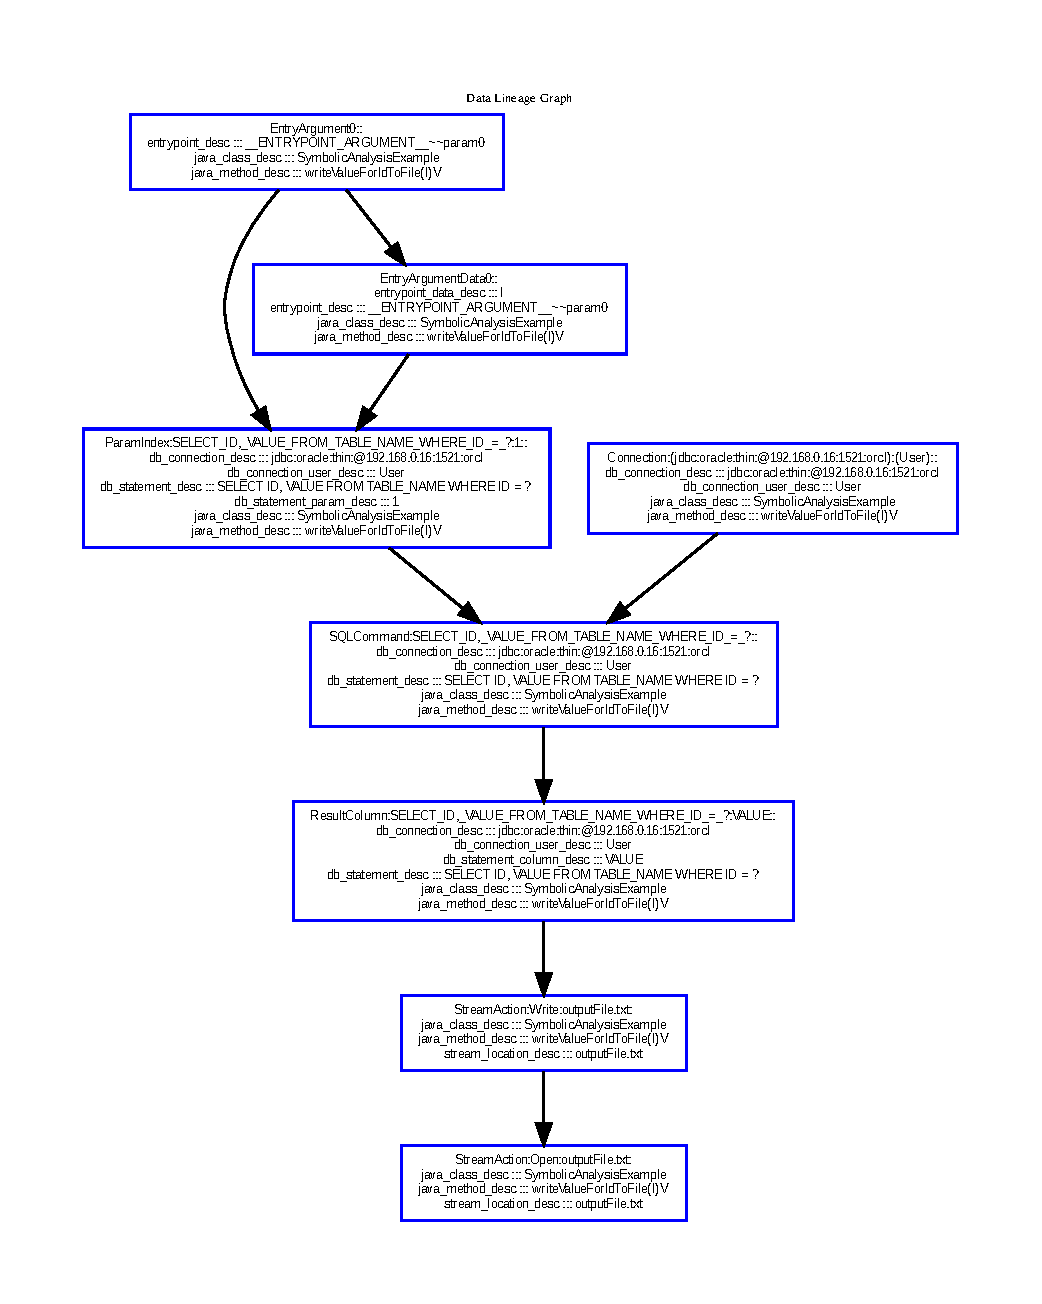
\includegraphics[trim={1cm 1cm 1cm 1.8cm},clip,width=\textwidth]{img/Examples2-writeValueForIdToFile.pdf}
  \caption{Visualization of data lineage graph}
  \label{frameworks:dbio:graph}
  \hspace{-15mm}
\end{figure}



\chapter{Data Lineage Analysis for Frameworks \label{chapter:implementation}}

In Chapter \ref{chapter:frameworks} we described Java frameworks
that are often used in applications to manipulate with data.

In Section \ref{frameworks:requirements} we described the key requirements
on the library to analyse data lineage of such applications.
The analysis library should:
\begin{itemize}
  \item Identify the data sources and sinks.
  \item Create correct and accurate data lineage in reasonable time.
  \item Work with the concrete values for Java primitives and \Code{String}s.
  \item Work with external files.
  \item Support the callback objects.
  \item Be easily extendible to support new frameworks.
\end{itemize}

In Section \ref{chapter:analysis:symbolicAnalysisLibrary} we described the
static program analysis approach used by the existing library
for creating data lineage of plain Java programs.
Using that library, data lineage can be created for Java I/O and JDBC API.

In this chapter, we will present our solution of data lineage analysis
for database frameworks - the \ToolName tool.
The \ToolName tool uses the Symbolic analysis library, which takes
care of the data flow propagation between sources and sinks.
The \ToolName tool implements features for identifying the sources
and sinks of data inside frameworks as plugins to the Symbolic analysis library.

We will discuss the design of the \ToolName tool and some technical details
of implemented Symbolic analysis library plugins.




\section{Symbolic Analysis Library Plugins}

In this section we describe the main ideas about plugin approach of our \ToolName tool.

When the Symbolic analysis library performs the program analysis,
the plugin handles the selected method calls on frameworks and provides
information about the data sources and data sinks to the library.

An input of a plugin is computed data flow information
about the receiver (\Code{this} object) and the method call arguments.
The Section \ref{chapter:analysis:algorithm} describes the Symbolic analysis algorithm
as iterative updating of method summaries until a fixpoint is reached.

The same approach applies for the plugins. At each iteration, the flow information
about the plugin inputs are computed by the library and based on their values,
plugin provides information about the data sources and sinks of a framework method call.




\section{Interface to Symbolic Analysis \label{chapter:implementation:interface}}

We proposed the general interface between Symbolic analysis library and its plugins.
Communication between the library and plugins is described in
Figure \ref{implementation:analysis-plugins-communication}.

\begin{figure}[p]
  \centering
  % trim - left lower right upper
  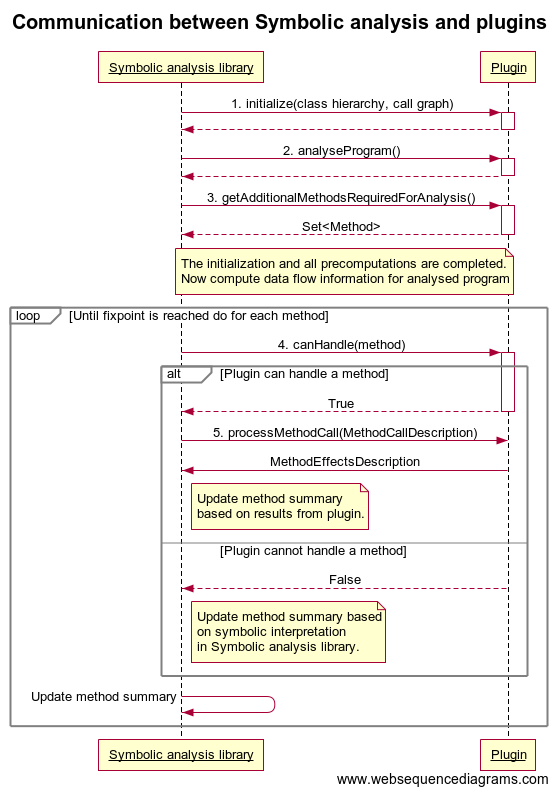
\includegraphics[trim={0cm 0.75cm 0cm 1.4cm},clip,width=\textwidth]{img/analysis-plugins-communication.png}
  \caption{Communication between Symbolic analysis and the plugins}
  \label{implementation:analysis-plugins-communication}
\end{figure}

In next sections we will describe all the interfaces used between the library and the plugins.



\subsection{FrameworkAnalysisPlugin}

The key interface for plugin to Symbolic analysis library is the\break
\Code{FrameworkAnalysisPlugin}.
The interface defines few methods that are used for communication between the library and plugins.
Here we describe their usage:
\begin{itemize}
  \item \Code{initialize} and \Code{analyzeProgram} initialize plugins
    and precompute some information from the provided call graph and class hierarchy
    of an analysed program.
  \item \Code{getAdditionalMethodsRequiredForAnalysis} specify framework methods that should
    be also analysed by the Symbolic analysis library, as the library does not
    analyse methods out of defined application package because of optimizations.
    Sometimes it is useful to analyse other framework methods
    (e.g. when there are many overloading methods that forward their calls to one method
    that can be handled by a plugin).
  \item \Code{canHandleMethod} and \Code{processMethodCall} query plugin whether method can be
    handled by the plugin and to compute flow information for such method.
  \item \Code{canProvideArgument} and \Code{getArgumentFlowInformation} provide flow information for
    an argument of a callback method.
  \item \Code{destroy} closes all plugin resources. The method is used at the end of analysis,
    when the fixpoint is reached.
\end{itemize}




\subsection{MethodCallDescription}

The class \Code{MethodCallDescription} serves as data flow information input for a plugin query
(the \Code{processMethodCall} method).
It holds the attributes for all method inputs
(for receiver (\Code{this} object) and all the method arguments)
and also flow information about the previously analysed callbacks.




\subsection{MethodEffectsDescription}

The class \Code{MethodEffectsDescription} serves as output of the\break
\Code{processMethodCall} method. It holds the output data flow information
and also identifies callbacks to be computed by the Symbolic analysis library.

Flow information are stored in the \Code{DataEndpointFlowInfo} object that
is described in the next section.



\subsection{DataEndpointFlowInfo}

The class \Code{DataEndpointFlowInfo} holds data flow information results
for an analysed method, such as:
\begin{itemize}
  \item Identification of the data source or sink.
  \item Mapping of fields in the resulting objects to data source or sink information (e.g. database column name).
    The results of a framework call can be returned by a method and also stored into a method attribute.
  \item Attributes for:
    \begin{itemize}
      \item Data source or sink
      \item Returned object
      \item Receiver (\Code{this})
      \item Method call arguments
    \end{itemize}
\end{itemize}

The data source and sink identification can be the SQL statement in case of database frameworks,
or the server identification, or other important information for data lineage.

Plugin can define its own attributes that can be used to identify any valuable information.
All of the attributes are then propagated using the Symbolic analysis library.




\section{JDBC API \label{implementation:jdbc}}

Implementation of Data Lineage for standard JDBC API in \Code{java.sql} package
is done using the Symbolic analysis library, as we show in the Section \ref{chapter:analysis:symbolicAnalysisLibrary}.

In this section we will describe our solution for \Code{DataSource} interfaces in \Code{javax.sql} package.
It is nowadays the preferred way of creating connections to database and the Symbolic Analysis
library do not handle such information.



\subsection{DataSource \label{implementation:dataSource}}

Database vendors usually provide \Code{DataSource} implementation, which still
needs some configuration about database - connection url, credentials and probably much more.

To identify target database, we need information about connection url and credentials. These properties
are usually set to \Code{DataSource} objects and from these calls, we can get
their values.

The plugins identify the methods where such information is set and return
the concrete values of used \Code{String}s for propagation by Symbolic analysis library.



\section{Spring JDBC Framework}

Spring JDBC Framework comes with approach of callbacks. It handles
all boilerplate code and calls user defined callback objects to do their job
and after finishing it, framework handles closing all resources that are not needed anymore.

When we looked to implementation of \Code{JdbcTemplate} class, we found out
that database calls are actually made only by 4 out of about 50 of its methods.
All the other methods only use them when executing queries.



\subsection{Callbacks}

As we said, callbacks are used just to wrap application logic and
separate it from the code for opening/closing connections, etc,
as was shown by previous example in Listing \ref{code:jdbcTemplate}.

When handling a particular method of the framework (e.g. the \Code{update}
method of \Code{JdbcTemplate} class in Listing \ref{code:jdbcTemplate}),
we needed to find a way how to say to the Symbolic analysis library that a plugin wants to
analyse that callback method. For that purpose, we use
field \Code{callbackMethodsToAnalyze} of the class \Code{MethodEffectsDescription} from the interface.
All callbacks have the method that is called in execution
and we just leave analysis library to analyse it and return
its data flow. After that, we append the resulting flow of the callback
to flow of our handled method.

We will demonstrate it on simple example of the \Code{insert} method from Listing \ref{code:jdbcTemplate}.
In the method, there is the call of the \Code{jdbcTemplate.update()} method
with two arguments - the SQL statement and the instance of the\break
\Code{PreparedStatementSetter}.

After data lineage analysis of the \Code{insert} method is done, we would like to know
that the \Code{id} and \Code{value} attributes of the \Code{DatabaseValue} instance
were arguments of the executed SQL statement.
However, Symbolic analysis library does not know that, inside of \Code{jdbcTemplate.update()},
the \Code{setValues} method of the \Code{PreparedStatementSetter} is called.

Our solution is that when the plugin is handling
\Code{jdbcTemplate.execute()} for the first time, it tells library
that it wants to analyse that \Code{setValues} call.
The next time the plugin already has all the information
about data lineage in the \Code{setValues}
and therefore it can propagate it to the result of the\break
\Code{jdbcTemplate.update()} call.




\section{MyBatis}

In chapter \ref{frameworks:myBatis} we showed classic use case of loading data from database
using the MyBatis framework. Now, we present solution of computing data lineage for this framework.



\subsection{Mapper interfaces}

First, it is necessary to find all the mapper interfaces.
To do this, we iterate all classes in class hierarchy and search 
for interfaces with methods annotated with MyBatis annotations,
or interfaces for which XML mapper definition exists.



\subsubsection{XML mapper files}

XML mapper file definition has the same name as the corresponding interface
(but .xml extension is used instead of .java), and lays in same directory.

We made a parser of such XML files that can get information about SQL statements
and mapping of columns to object fields.

Parser supports reusable SQL fragments. Each fragment has its own ID,
so it is easy to find correct one and include it into query.

Parser also supports dynamic SQLs. As we do not know which conditions are valid
at runtime, we made a simplification that we always use just first branch that
was seen in the code.
We also cannot determine the size of an input collection, so the parser provides no expansion.



\subsubsection{Annotated mapper classes}

When mappers use annotations, it is quite simple to get all data needed
from WALA. We know that an SQL statement is always stored in annotations
\Code{@Select}, \Code{@Insert}, \Code{@Delete} or \Code{@Update}
and queries are stored in plain \Code{String} array.
Queries can also contain dynamic SQL as in XML definitions.

For mapping result object the \Code{@Results} annotation is used with \Code{@Result}
for every column to object property mapping definition.
Mapping can be done using \Code{@ConstructorArgs}, when columns are mapped
to arguments of a constructor. In that case, the plugin unfortunately does not know
the name of target property, as arbitrary code can be executed in constructor\footnote{
  Arbitrary code can be executed also in setters, but it is usually used
  just as setting new reference of a property.
}.

Framework can provide result of an SQL query in two ways:
\begin{enumerate}
  \item As a return statement of a mapper method.
  \item As a method argument property.
\end{enumerate}

In all previous mapper examples, we use the first approach, where result
is returned from method in return statement.

However, when calling database procedure, we can define its output arguments
and framework fill result values into that method argument.
It can be \Code{Map<String, Object>} object (where mapper references to key in that map),
or any arbitrary object (where mapper references field, in which result will be stored).

Listing \ref{code:mybatis:advanced:map} illustrates the use of such \Code{Map} as
input and also output method argument.
The database call of \Code{DB\_PROCEDURE} has two arguments.

First, the input integer argument, takes value of the \Code{id} key from the map.
Second, the output cursor argument, is created by MyBatis and perform database procedure call.
The cursor is then transformed to list of target objects
with result map \Code{resultMap} and stored to the same map under the key \Code{result}.

\InsertCode{h}{code/mybatis-output-arguments.tex}

There also exist more advanced features of MyBatis\footnote{
  Such as using provider classes to create SQL queries (\Code{@SelectProvider}, $\ldots$),
  generating IDs from sequence (\Code{@SelectKey}) and using them in queries,
  generating maps from objects (\Code{@MapKey}),
  associations for attribute classes (\Code{@One} or \Code{@Many}),
  mixing XML and annotation mappers (e.g. define \Code{<resultMap>} in XML and reference it
  using \Code{@ResultMap} annotation)}
but we do not handle them. All of them can be added as new functionality in future development,
if needed.




\subsection{Database connection configuration}

Configuration of MyBatis can be done in two ways, using XML configuration file
or in Java using \Code{Configuration} class. Second way needs no more attention,
as we use \Code{DataSource} classes that are already handled in section \ref{implementation:dataSource}.

To handle XML configuration, our plugin needs to parse configuration file and find \Code{<dataSource>}
section and its \Code{driver}, \Code{url} and \Code{username} properties. All this
information we need for identifying target database.




\section{Kafka}

In section \ref{frameworks:kafka} we demonstrated the main use cases
for data manipulation (producing or consuming) using Kafka framework.
In this section, we show how data lineage for these examples can be computed
using our plugin. In our work, we focused only on Consumer and Producer APIs,
as the other two (Stream and Connector APIs) are much more advanced to use.

The plugin identifies the used Kafka server which is used in application to communicate with.
It also identifies the methods that are used to set Kafka topics
and the methods that are used to send and receive a data.

Together, the used server, topic and the place where data are produced and consumed,
are the main data lineage information about the sources and sinks of a data.




\subsection{Callbacks}

Kafka Framework uses callbacks to asynchronously notify application.
It can be callbacks to notify about performed operation result (like in case of sending data),
or to notify about some state changes.

As in case of callbacks in Spring JDBC Framework, the plugin tells
the Symbolic analysis library to analyse the data flow in such callback method
and then plugin propagate computed data flow information 
to the result of handled method.




\subsection{Properties}

Kafka Framework uses Java \Code{Properties} to its configuration.

\Code{Properties} can be set in Java code (like it was done in
Listing \ref{code:kafka:consumer} and Listing \ref{frameworks:kafka:producer}).
They can be also loaded from external file like in next code:
\begin{lstlisting}[language=JavaSnippet]
        new Properties().load(new FileReader("file.txt"));
\end{lstlisting}

When the \Code{Properties} values are set only using Java, the concrete
values are resolved by Symbolic analysis library.

However, the library does not support the external files for loading properties.
It provides only the stream identification (name of used file, \uvodzovky{System.in}, etc.).

If there exists a file with such identification, plugin loads its properties and
tries to resolve what Kafka server was used in application.




\chapter{Evaluation \label{chapter:results}}

In this chapter, we provide results of our \ToolName tool.
The tool provides implementation of plugins for three frameworks
that are used for manipulatin data - Spring JDBC, MyBatis and Kafka.
It also provide implementation for the identification of many types of databases
through \Code{DataSource} interface.

The \ToolName tool can also visualize data flow of JDBC and I/O API that was
implemented in Symbolic analysis library and is not part of our work.

In next sections, we evaluate results of our \ToolName tool for each of the selected frameworks.
In the end, we discuss limitations of the current solution and discuss
the requirements from \ref{frameworks:requirements}, whether they were
fullfilled by our \ToolName tool.




\section{Data Flow Graph Visualizations for Frameworks}

In this section we present some data flow visualizations
for example programs that were presented in previous sections.

\TODO{Vlozit a popisat obrazky}



\section{Limitations of the \ToolName Tool \label{chapter:results:limits}}

There are few negative aspects in our \ToolName tool implementation.
We try to point them out in next list:
\begin{enumerate}
  \item \textbf{Slow data lineage computation.} \\
    The data lineage computation tests in our project last from
    a few tens of second to a few minutes. It depends on the
    number of used libraries, their complexity and also from complexity
    of analysed application.
  \item \textbf{There can be many algorithm iterations until fixpoint is reached.} \\
    The Symbolic analysis library computes method summaries iteratively until
    fixpoint is reached - when there are no changes in the method summaries.
    The number of iterations also depends on the number of methods in the analysed program.
  \item \textbf{Some inaccuracies can occur based on used over-approximation algorithm.} \\
    The Symbolic analysis library computes over-approximation (e.g. when accessing
    an element of an array or collection, all elements are considered as output).
  \item \textbf{Disadvantages of static analysis.} \\
    Many disadvantages comes with the usage of static analysis,
    when values are computed dynamically based on the external inputs.
\end{enumerate}



\section{Fulfillment of the Assignment}

\TODO{Alebo nazvat diskusia nad splnenim zadania?}

In the Section \ref{frameworks:requirements} we pointed out the requirements
on the library to be able to successfully compute the data lineage of
applications that use frameworks for accessing the data.

In the next list we try to explain how the requirement is fullfilled (or not)
by the \ToolName tool:
\begin{enumerate}
  \item \textbf{Analysis of whole Java application.} \\
    Our tool analyse both application and its dependencies
    to distinguish all the data flows. The used WALA framework
    needs all dependencies to create correct call graph.
  \item \textbf{Identifying the sources and sinks.} \\
    The plugins for Symbolic analysis library identify the sources and sinks
    of an analysed application when the corresponding frameworks are used.
  \item \textbf{Correctness, accuracy and efficiency of computing data lineage.} \\
    We explained some limitations of our \ToolName tool in the Section \ref{chapter:results:limits}.
    The data lineage computation can take quite long time, depending on the complexity of an analysed
    application and the number of used libraries.
    However, it is expected, that analysis of a huge program with many library dependencies
    will run slower than the analysis of other small Java application.
    As the tests in the \ToolName tool show, the data lineage is computed
    in few minutes, therefore the tool is usable in practice.
  \item \textbf{Work with external files.} \\
    The external configuration files are often handled by our plugins for the Symbolic analysis library.
  \item \textbf{Use concrete values.} \\
    The Symbolic analysis library always tries to resolve actual values of Java primitives and
    \Code{String}s. However, even if in many cases the concrete values cannot be determinated,
    the data flow between sources and sinks are preserved.
    As the frameworks often use external files for storing its data, that files can be often read
    by the \ToolName tool to evaluate the data sources and sinks identifiers.
  \item \textbf{Handle callbacks.} \\
    The Symbolic analysis library supports also computing the data flow in callbacks.
  \item \textbf{Easy extendability.} \\
    We proposed the pluggable architecture for the Symbolic analysis library.
    We demonstrated the possibilities that result from the changed architecture
    on several library plugins. Plugins identify the data sources and sinks
    of used data processing frameworks.
\end{enumerate}



\chapter*{Záver}
\addcontentsline{toc}{chapter}{Záver}

TODO Nejaky zaver


%%% Seznam použité literatury
%%% Seznam použité literatury (bibliografie)
%%%
%%% Pro vytváření bibliografie používáme bibTeX. Ten zpracovává
%%% citace v textu (např. makro \cite{...}) a vyhledává k nim literaturu
%%% v souboru literatura.bib.
%%%
%%% Příkaz \bibliographystyle určuje, jakým stylem budou citovány odkazy
%%% v textu. V závorce je název zvoleného souboru .bst. Styly plainnat
%%% a unsrt jsou standardní součástí latexových distribucí. Styl czplainnat
%%% je dodáván s touto šablonou a bibTeX ho hledá v aktuálním adresáři.

\bibliographystyle{plainnat}    %% Autor (rok) s anglickými spojkami
% \bibliographystyle{unsrt}       %% [číslo]

\renewcommand{\bibname}{References}

%%% Vytvoření seznamu literatury. Pozor, pokud jste necitovali ani jednu
%%% položku, seznam se automaticky vynechá.

\bibliography{literatura}

%%% Kdybyste chtěli bibliografii vytvářet ručně (bez bibTeXu), lze to udělat
%%% následovně. V takovém případě se řiďte normou ISO 690 a zvyklostmi v oboru.

% \begin{thebibliography}{99}
%
% \bibitem{lamport94}
%   {\sc Lamport,} Leslie.
%   \emph{\LaTeX: A Document Preparation System}.
%   2. vydání.
%   Massachusetts: Addison Wesley, 1994.
%   ISBN 0-201-52983-1.
%
% \end{thebibliography}


%%% Obrázky v bakalářské práci
%%% (pokud jich je malé množství, obvykle není třeba seznam uvádět)
\listoffigures

%%% Tabulky v bakalářské práci (opět nemusí být nutné uvádět)
%%% U matematických prací může být lepší přemístit seznam tabulek na začátek práce.
%\listoftables

%%% Přílohy k bakalářské práci, existují-li. Každá příloha musí být alespoň jednou
%%% odkazována z vlastního textu práce. Přílohy se číslují.
%%%
%%% Do tištěné verze se spíše hodí přílohy, které lze číst a prohlížet (dodatečné
%%% tabulky a grafy, různé textové doplňky, ukázky výstupů z počítačových programů,
%%% apod.). Do elektronické verze se hodí přílohy, které budou spíše používány
%%% v elektronické podobě než čteny (zdrojové kódy programů, datové soubory,
%%% interaktivní grafy apod.). Elektronické přílohy se nahrávají do SISu a lze
%%% je také do práce vložit na CD/DVD.
%\chapwithtoc{Prílohy}

\openright
\end{document}
